%!TeX root = 6-perspectives.tex
\documentclass[main]{subfiles}

\begin{document}

\chapter{Towards the next generation of screening}
\vspace*{-1\baselineskip}

\section{Limits of the current screening methodologies}

As presented in the review of different methodologies for screening materials in Chapter 1, it is a common practice to screen for a specific metric, such as selectivity, permselectivity, or capacity, depending on the targeted application. Attempts to screen for materials that exhibit high selectivity while also possessing a good capacity are increasingly prevalent in current research\autocite{Chung_2019,Zhang_2022,Solanki_2020}. For instance, improvements can be made in selectivity screening regarding calculation efficiency and the accuracy of molecular description. The previous chapters primarily focused on enhancing efficiency by exploring various techniques for sampling adsorption energy and comparing their computational time and accuracy. Furthermore, the screening procedure was enhanced by incorporating transport properties. Additionally, alternative calculation strategies were explored and developed to increase the efficiency of screening diffusion coefficients (e.g., transition state detection, machine learning models) compared to computationally expensive conventional methods (MD simulations).

To address the limitations of the current methodologies for adsorption screening, a more accurate physical description of the nanoporous system is required. For example, the rigid nature of structures in most screening procedures can sometimes lead to misleading results, as materials may appear to have high selectivity, but exhibit decreased computed selectivity values due to their flexible nature. Considering flexibility in the analysis can modify the rankings obtained from previous screenings and potentially identify other top materials. Another physical property that can significantly impact the screening results is polarization. In the case of adsorbates like xenon and krypton, the difference in polarizability plays a crucial role in the separability of these gases using adsorbent materials. A more precise characterization of this property has the potential to completely alter the screening outcomes. Notably, the best experimental materials often feature decorations with polar groups (Ref.\cite{Li_2019}) or possess open metal sites (Ref.\cite{Pei_2022}), although these criteria were not deemed essential in the current screenings.

This final chapter will explore prospective studies focusing on three main research areas: (i) the efficiency improvement of the calculation of transport properties, (ii) the adsorption calculations in flexible frameworks for screening purposes, and (iii) a more accurate description of polarization interactions in molecular simulations.

\section{Future developments on transport properties}

During the Ph.D. project, the transport properties were thoroughly studied using MD simulations and an ML model primarily based on the PLD and a proxy of the diffusion activation energy. This approach provides very promising results as it significantly accelerates the evaluation of diffusion coefficient values. However, when employing an ML-based approach, the generalizability to other types of systems cannot be guaranteed. To create a simulation that is faster than MD simulations while ensuring higher accuracy and reliability than the ML-based approach, the next steps involve completing the development of the diffusion coefficient calculation code based on the transition state theory (TST) and kinetic Monte Carlo (kMC) simulations. This code is currently in its final stages of development, as explained in the preceding chapter. Once this new approach is developed, it can provide diffusion coefficients that can be utilized in breakthrough modeling software for comparison with experimental data. The subsequent section presents a description of such software, exploring the perspectives offered by RUPTURA\autocite{Sharma_2023}.

\subsection{Final development of the optimized version of TuTraST}

The diffusion calculation code, based on the TST and kMC, already possesses several capabilities: (i) calculating the energy grid using the GrAED algorithm, (ii) identifying connected components or clusters through a breadth-first search algorithm, (iii) detecting channels using a simple all-direction scanning algorithm on the identified clusters, and (iv) determining the energy barrier by utilizing (ii) and (iii) in a loop over the energy values. The energy barrier of a particular channel is defined as the energy at which the channel reconnects with at least one channel connected through at least one direction.

To finalize the implementation of the algorithm, the final step entails detecting the transition state surfaces that separate different clusters. This final mapping, which establishes basins connected by transition surfaces, can then be used in a simple kMC scheme to determine the diffusion coefficient. In the original work by Mace et al.\autocite{Mace_2019}, the authors achieved the growth of clusters with energy values below $E\e{min}+i\delta E$ by incrementally expanding them layer by layer until they reached energy values below $E\e{min}+(i+1)\delta E$. When a point from a layer of one cluster touches another cluster, that point can be considered a transition point if the energy gap is sufficiently high. Otherwise, the two clusters merge to form a single cluster. The loop over the energy values is employed to restrict the transition points to the range between $E\e{min}+(i)\delta E$ and $E\e{min}+(i+1)\delta E$. Upon reflection, the layer-by-layer growth method does not identify the highest energy point in a given direction, as conventionally defined for transition states. Instead, it detects points that are equidistant from the surfaces of two previous clusters. Both definitions are equivalent if the value of $\delta E$ is infinitely small.

To avoid using a computationally expensive layer-by-layer growth, an alternative possibility is to assign labels using a breadth-first search approach. The boundary points between two connected components can be determined as the points that are ``equidistant'' to the clusters. The definition of equidistant depends on the definition of distance. It can be directly defined based on the grid cells, corresponding to the Manhattan distance. However, this distance metric may be sensitive to the angle values of the unit cell --- a tilted cell could introduce bias in the neighbor search towards a particular direction. To overcome this limitation, a Cartesian coordinate grid would be necessary, and a bucket queue prioritized according to Cartesian distances would replace the standard queue based on grid neighbors (as presented in section~\ref{sct:tutrast}).

In future research, the focus of the thesis will be on studying different approaches: layer-by-layer growth, breadth-first search with a standard queue, or a bucket queue prioritized using Cartesian distances. The objective is to compare their performance in terms of time and accuracy.

\subsection{Connection to the breakthrough experiments}

The relevance of the diffusion coefficient calculated by these methods can only be reliably validated through a comparison with experimental data. However, accessing the diffusion coefficient inside a nanoporous material can be challenging through experiments. The shape of the experimental breakthrough curves provides a glimpse of the kinetic performance. An indirect comparison can be achieved by generating breakthrough curves from the computed diffusion coefficients and comparing them with experimental data. To separate the kinetics from the thermodynamics of the adsorption process, a breakthrough model based on both the computed transport properties and the experimental isotherm data might be necessary.

\begin{figure}[ht]
  \centering
  \begin{subfigure}[b]{0.5\textwidth}
    \centering
    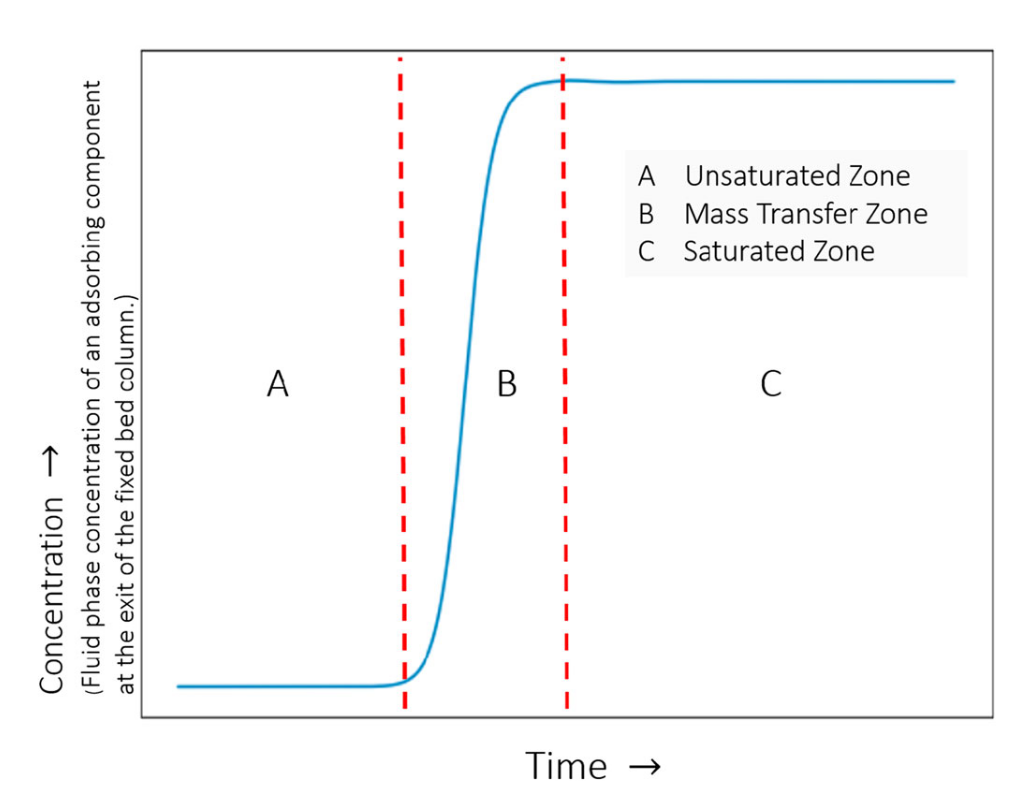
\includegraphics[width=\textwidth]{figures/6-perspectives/breakthrough_cuve_zones.png}
    \caption{Breakthrough curve zones}\label{fgr:breakthrough_zones}
  \end{subfigure}
  \hfill
  \begin{subfigure}[b]{0.4\textwidth}
    \centering
    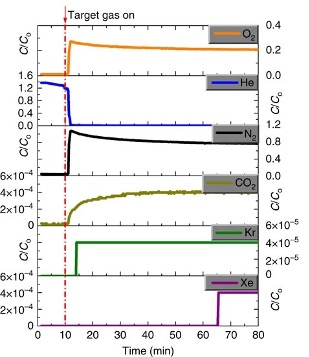
\includegraphics[width=\textwidth]{figures/6-perspectives/sbmof_breakthrough.jpg}
    \caption{SBMOF-1 experimental breakthrough}\label{fgr:sbmof_breakthrough}
  \end{subfigure}
  \caption{ (a) Different zones in a breakthrough curve reprinted from the open-access article~\cite{Sharma_2023}. (b) Experimental breakthrough curves in SBMOF-1 for a gas mixture with 400 ppm Xe and 40 ppm Kr balanced with dry air. Reprinted with permission from Ref.~\cite{Banerjee_2016} copyright \copyright\ 2016 Springer Nature. }\label{fgr:breakthrough}
\end{figure}

A breakthrough curve can be broken down into three different zones: an unsaturated zone, a mass transfer zone, and a saturated zone, as shown in Figure~\ref{fgr:breakthrough_zones}. The mass transfer zone can be qualitatively interpreted as a consequence of the different transport properties. For instance, The breakthrough curves are based on quantities obtained from an adsorption isotherm fit, and mass transfer properties such as the self-diffusion coefficient and material surface diffusion (Knudsen diffusion).\autocite{Sharma_2023}. This tool has the potential to generate breakthrough curves and compare them to experimental curves. When the isotherm fitting properties are derived from experimental calculations, the only variable remaining is the mass transfer term. In this case, this tool can be used to qualitatively validate a calculated self-diffusion coefficient value.

Using SBMOF-1 as an example (Figure~\ref{fgr:sbmof_breakthrough}), a rather slow mass transfer can be associated with \ce{CO2}, while the mass transfer corresponds to a vertical line for the other components, indicating fast diffusion rates. Consequently, there is a diffusion limitation for \ce{CO2} but not for the other adsorbates in the SBMOF-1 material. However, the absence of diffusion limitation for xenon sheds light on an apparent inconsistency with the diffusion coefficient calculated by an MD simulation ($3\times 10^{-8}$\si{\square\cm\per\s}). The next section on the flexible nature of SBMOF-1 offers a reasonable explanation for this discrepancy between the experimental and simulated evaluations of the diffusion.

\section{Screening of flexible materials}

The preference for studying rigid frameworks in computational studies is due to the high complexity associated with the simulation of the dynamics of a flexible framework. Given the considerable cost associated with simulating a grand canonical ensemble using MC methods, the simulation of a flexible framework would be even more computationally expensive, as it would require relaxation of the volume and simulation of an osmotic ensemble ($\mu$,$P$,$T$), which necessitates additional MC moves on the volume of the unit cell itself.\autocite{Bousquet2012}. Although this type of MC simulation describes more accurately every aspect of flexibility, including intrinsic flexibility due to thermal agitation and adsorbate-induced flexibility, it is prohibitively time-consuming in large-scale screening procedures. Therefore, it is more practical to use this type of simulation as a precise method to confirm the properties of a few top materials.

In order to incorporate flexibility effects in the screening procedure at a minimal computational cost, another approach consists in using a set of rigid structures that reflects the structural diversity generated by the thermal agitation of the nanoporous material. A first study on the effect of this intrinsic flexibility on the Xe/Kr selectivity suggests that some materials could lose selectivity due to the less favorable pore size as the structure vibrates.\autocite{Witman_2017} For instance, it was found that the differences between the experimental and theoretical Xe/Kr selectivity of \texttt{KAXQIL}\autocite{KAXQIL} are caused by its intrinsic flexibility, which questions the performance ranking obtained through rigid-framework screening. In this section, the study of Witman et al.\autocite{Witman_2017} on a screening of intrinsic flexibility will be detailed, with a specific focus on the case of \texttt{KAXQIL}. The subsequent flexibility study will be based on the structural diversity among similar deposited experimental structures. Notably, there exist a dozen different structures with the same chemical nature as \texttt{KAXQIL}, but with very distinct structural characteristics depending on the loaded adsorbate, which suggests an adsorbate-induced flexibility in addition to the previously studied intrinsic flexibility. 

\subsection{Snapshot method}

\subsubsection{Methodology}

To model the dynamics of the framework, Witman et al.\ used the UFF forcefield to describe the non-electrostatic framework bond potentials, except for the metal bonding. For the bond dynamics around the metal, a harmonic equilibrium potential was fixed around the values extracted from the experimental structure. For this reason, this forcefield definition is referred to as the UFF-fix-metal (UFF-FM). In addition of the Lennard-Jones description, the point charge Coulomb interactions were described using the standard Ewald summation technique based on the charges calculated by the density derived electrostatic and chemical (DDEC) method.\autocite{manz2010chemically} Using this forcefield, the authors carried out a systematic snapshot generation of the structures from the CoRE MOF 2014 database with pre-calculated DDEC charges. These snapshots were then utilized to determine the Xe and Kr Henry constant values for the flexible structures, as well as the infinite dilution Xe/Kr selectivity. The study revealed that the flexible selectivity was lower for {95\%} of the materials with a rigid selectivity over $25$ (as shown in Figure~\ref{fgr:underestimated_rigid}), which suggests an overestimation of the top performing materials. Furthermore, the effect of flexibility is much more important for materials with smaller pore sizes due to the increased intensity of interactions at shorter distances.


\begin{figure}[ht]
  \centering
  \begin{subfigure}[b]{0.32\textwidth}
    \centering
    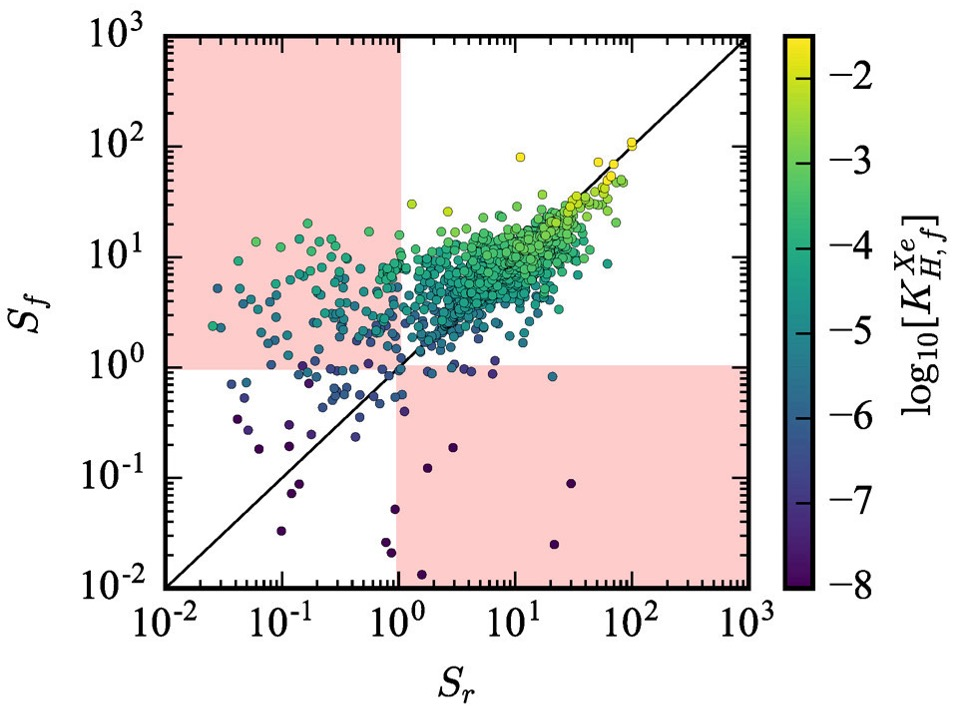
\includegraphics[width=\textwidth]{figures/6-perspectives/s_f-s_r.jpg}
    \caption{Flexible \emph{vs.} Rigid}
  \end{subfigure}
  \hfill
  \begin{subfigure}[b]{0.3\textwidth}
    \centering
    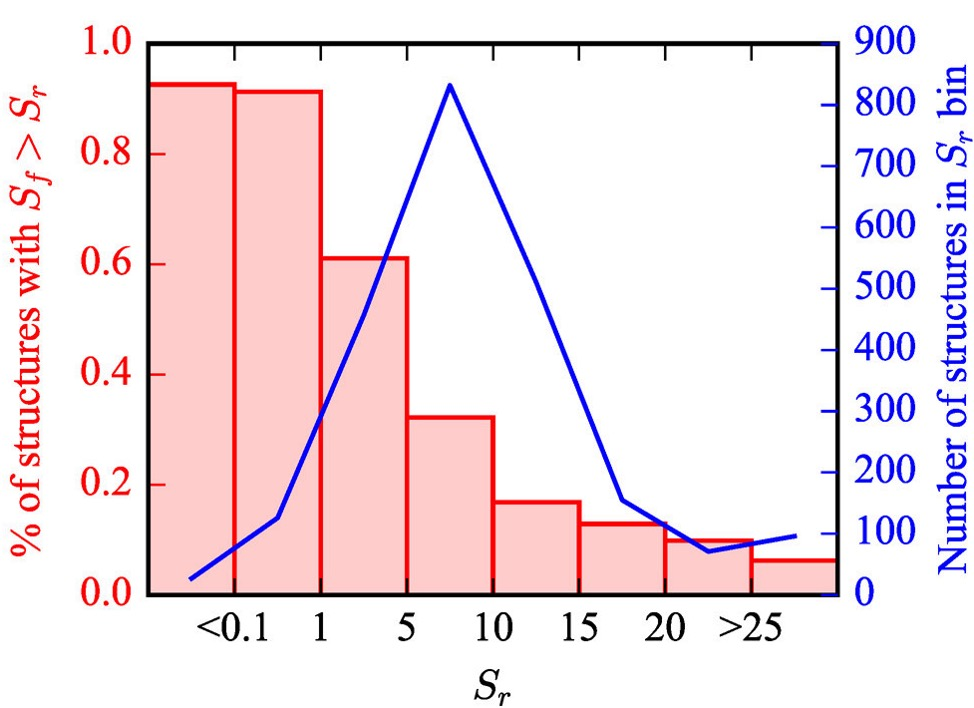
\includegraphics[width=\textwidth]{figures/6-perspectives/histogram_flex.jpg}
    \caption{selectivity underestimation}\label{fgr:underestimated_rigid}
  \end{subfigure}
  \hfill
  \begin{subfigure}[b]{0.32\textwidth}
    \centering
    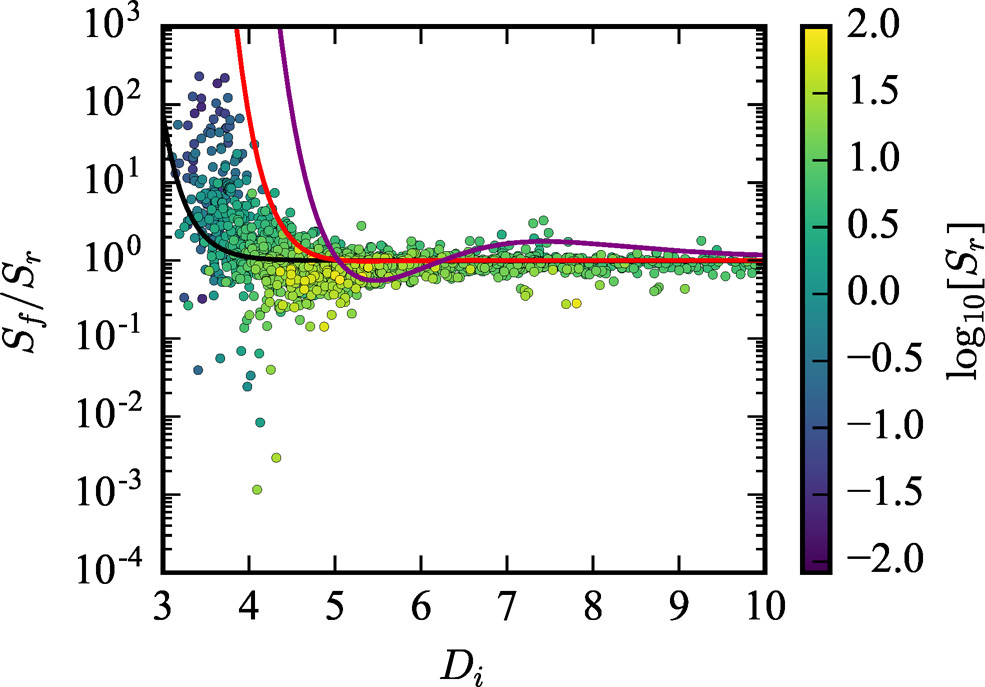
\includegraphics[width=\textwidth]{figures/6-perspectives/s_ratio_LCD.jpg}
    \caption{Flexibility effect \emph{vs.} LCD}
  \end{subfigure}
  \caption{ (a) A scatter plot of the flexible selectivity against the rigid selectivity labeled by the log$_10$ of the flexible Xe Henry constants. (b) Barplot of the fraction of the underestimated selectivity ($s_f>s_r$) for different categories of materials going from the least selective ones to the most selective ones ($s_r>25$). (c) Effect of the flexibility measured using the ratio $s_f/s_r$ as a function of the largest included sphere diameter. The line plots corresponds to analytical modeling of the effect that will not be detailed here. Reprinted with permission from the original paper~\cite{Witman_2017} copyright \copyright\ 2017 American Chemical Society. }\label{fgr:flexibility_study}
\end{figure}

Turning to the issue of flexibility in \texttt{KAXQIL}, the authors used several methods to evaluate its effect on the Xe and Kr Henry constants and the Xe/Kr selectivity. For instance, they leveraged an alternative description of the metal--ligand bond utilizing a cationic dummy model (UFF-CDM) and an \emph{ab initio} MD simulation performed using the PBE DFT function,\autocite{Perdew_1996} with a Grimme's D3 van der Waals correction\autocite{Grimme_2010} (PBE+D3). Each of these three methods was employed to generate approximately $30$ snapshots, which were subsequently used to determine the flexible framework's adsorption properties for \texttt{KAXQIL}.

The authors found that the lower experimental selectivity value of $16$, as compared to the UFF-determined value, could be partially attributed to a flexibility effect. As shown in Table~\ref{table:witman_sbmof}, the selectivity value decreases from $54$ to $25$ when changing from a rigid to a flexible structure. The selectivity evaluated using the standard UFF forcefield on a rigid SBMOF-1 structure is considerably higher than the selectivity obtained when considering snapshots of a vibrating structure. Although the \emph{ab initio} MD method should provide the closest representation of the actual dynamics, it did not fully capture the phenomenon due to the dependence on system size. Typically, multiple unit cell replications are required to observe crystallographic deformations. Moreover, the UFF forcefield does not provide a perfect picture of the interaction energies at play in the system. Nonetheless, this study establishes an overall trend by attributing the discrepancies between experimental and theoretical data to the rigidity hypothesis.

\begin{table}[t]
  \centering
  \small
  \begin{tabular}{|l|c|c|c|c|}
  \hline
    Data source & Flexible &  Xe Henry Constant &  Kr Henry Constant &  Xe/Kr \\
      & structure &  \si{\mmol\per\g\per\Pa} &  \si{\mmol\per\g\per\Pa} &  selectivity \\
  \hline
    Experimental data\autocite{Banerjee_2016} & maybe &  $3.84\,10^{-4}$ &  $2.37\,10^{-5}$ &  $16$ \\
  \hline
    Rigid structure SBMOF-1\autocite{Banerjee_2016} & no &  $1.45\,10^{-2}$ &  $2.70\,10^{-4}$ &  $54$ \\
    PBE+D3 (2,2,1 unit cell) & yes &  $6.80\,10^{-3}$ &  $1.77\,10^{-4}$ &  $38$ \\
    UFF-FM & yes &  $6.24\,10^{-3}$ &  $1.67\,10^{-4}$ &  $37$ \\
    UFF-DCM & yes &  $3.18\,10^{-3}$ &  $1.28\,10^{-4}$ &  $25$ \\
  \hline
\end{tabular}
\caption{ Results of the flexibility analysis carried out by Witman et al., flexibility reduces the values originally calculated in a rigid structure. Reproduced with permission from the original paper~\cite{Witman_2017} copyright \copyright\ 2017 American Chemical Society.}\label{table:witman_sbmof}
\end{table}

Although this approach does not fully describe the flexibility effect on the selectivity value, it can rapidly identify a weakness in the rigidity hypothesis, thereby warning of a possible over- or under-estimation of the selectivity. This can lead to the wrongful identification of a material as the best or the missed opportunity of finding a better material. The main advantage of this technique is its relative speed compared to an osmotic ensemble Monte Carlo simulation.\autocite{Bousquet2012} However, the imperfect description of the intrinsic flexibility as the only phenomenon at play is its main drawback. For instance, the following discussion will focus on some adsorbate-induced effects that were outlooked but can be retrieved by utilizing multiple works on the same SBMOF-1 material. This approach avoids the issues around simulating the flexible structure, as the reasoning is solely based on experimentally observed structural changes.


\subsection{Experimental database approach}

According to original paper on SBMOF-1,\autocite{Banerjee_2016} the theoretical selectivity calculated by UFF is around $70.6$. However, the experimental selectivity is significantly lower, around $16$. To solve this difference, Witman et al.\ used a snapshot-based method to evaluate the effect of selectivity. The intrinsic flexibility lowers the selectivity, which aligns with explaining the difference in selectivity, but it does not appear to capture the whole picture. 

For instance, the observed discrepancies could also be explained by the deformation induced by the loading of adsorbate inside the material. For instance, experimentally, a structure is often not empty when resolved by X-ray, and molecules are actually loaded inside. As shown in Table~\ref{table:sbmof}, the structure that was originally published for its good \ce{CO2}/\ce{N2} selectivity\autocite{Yeh2012,Banerjee2012} was also tested for water adsorption, and two different structures emerged from this study: \texttt{KAXQOR} and \texttt{KAXQIL}. The first one is loaded with either air or \ce{CO2}, and the structure does not seem to be stretched as much (low LCD values around \SI{4.5}{\angstrom}). The second one, on the other hand, is filled with water that forms big clusters inside the pores and therefore stretches the pore size towards higher values (high LCD values around \SI{5.0}{\angstrom}). Looking at the structures resolved in the \emph{Nature Communications} study\autocite{Banerjee_2016}, depending on the adsorbate (UQEFAZ for krypton or UQEFED for xenon), the LCD and PLD values change in the first order according to the size of the adsorbate as illustrated in Figure~\ref{fgr:stretch}. There are, of course, other effects, like the clustering mentioned for water, but also less expected effects such as the orientation of the adsorbate inside the structure. 

\begin{table}[t]
\centering
\setlength\extrarowheight{2pt}
\small
\begin{tabular}{|l|r|c|c|c|c|c|}
  \hline
  Experimental structure & Adsorbate in &  Selectivity & $K\e{H}\ex{Xe}$ &  LCD  &  PLD  &  Xe Diff. \\
  CCSD ref.~code & the structure &  $s\ex{Xe/Kr}_0$ &  (\si{\mmol\per\g\per\pascal}) &  (\si{\angstrom}) &  (\si{\angstrom}) & Coeff. \si{\square\cm\per\s} \\
  \hline
  \texttt{KAXQOR01}\autocite{Yeh2012} & Not specified & 101 & 3$\times$10\ex{-2} &  4.99 & 3.66 & 3$\times$10\ex{-09} \\
  \texttt{KAXQOR}\autocite{Banerjee2012} & Not specified & 22 & 4$\times$10\ex{-3} & 4.51 & 4.04 & 7$\times$10\ex{-06}  \\
  \texttt{KAXQIL}\autocite{Banerjee2012} & H$_2$O & 104 & 3$\times$10\ex{-2} & 5.12 & 3.77 & 3$\times$10\ex{-08} \\
  \texttt{QUXRIM}\autocite{Banerjee2016hydro} & hexane &  52 & 1$\times$10\ex{-2} & 4.75 & 4.31 & 3$\times$10\ex{-05}  \\
  \texttt{QUXRUY}\autocite{Banerjee2016hydro} & hexane &  96 & 3$\times$10\ex{-2} & 4.91 & 3.57 & 9$\times$10\ex{-10} \\
  \texttt{QUXROS}\autocite{Banerjee2016hydro} & hexane &  99 & 3$\times$10\ex{-2} & 5.00 & 3.66 & 5$\times$10\ex{-09}  \\
  \texttt{QUXREI}\autocite{Banerjee2016hydro} & hexane & 101 & 3$\times$10\ex{-2} & 5.02 & 3.67 & 7$\times$10\ex{-09}  \\
  \texttt{QUXRAE}\autocite{Banerjee2016hydro} & hexane & 100 & 3$\times$10\ex{-2} & 5.03 & 3.68 & 7$\times$10\ex{-09}  \\
  \texttt{QUXQUX}\autocite{Banerjee2016hydro} & butane & 103 & 3$\times$10\ex{-2} & 5.17 & 3.83 & 1$\times$10\ex{-07}   \\
  \texttt{QUWYEO}\autocite{Banerjee2016hydro} & butane & 100 & 3$\times$10\ex{-2} & 4.99 & 3.65 & 5$\times$10\ex{-09} \\
  \hline  
  \texttt{UQEFAZ}\autocite{Banerjee_2016} & krypton & 23 & 5$\times$10\ex{-3} & 4.53 & 4.08 & 5$\times$10\ex{-06}   \\
  \texttt{UQEFED}\autocite{Banerjee_2016} & xenon & 63 & 3$\times$10\ex{-2} & 4.89 & 3.54 & 1$\times$10\ex{-11}   \\
  \hline
  \end{tabular}
  \caption{ Structural, adsorption and transport properties of structures in the CSD database that are similar to SBMOF-1\autocite{Banerjee_2016}. The last structures actually correspond to the structures resolved in the paper presenting SBMOF-1 in Nature Communications. We can note the structural diversity that induces this diversity of properties. (The pore sizes are calculated using the CCDC radii definition.) }\label{table:sbmof}
\end{table}

As shown in Figure~\ref{fgr:ads_config}, the orientation of the hexane molecule inside the material seems to favor either a configuration with a large LCD and a low PLD (\texttt{QUXRUY}), or a slightly lower LCD with a slightly higher PLD (\texttt{QUXRIM}). The material configurations are, however, slightly different from the ones observed with \texttt{KAXQOR} or \texttt{KAXQIL}. 

\begin{figure}[ht]
  \centering
  \begin{subfigure}[b]{0.45\textwidth}
    \centering
    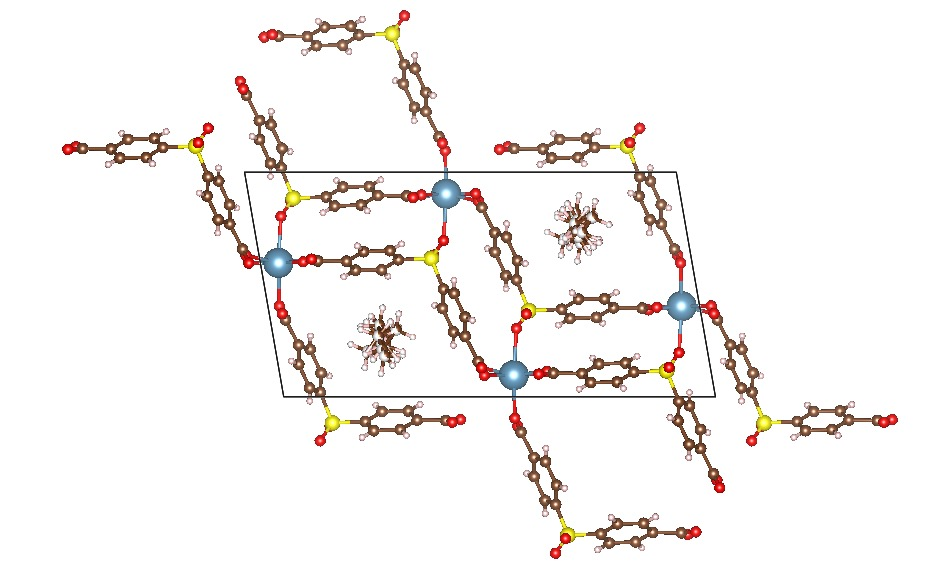
\includegraphics[height=0.6\textwidth]{figures/6-perspectives/QUXRIM.jpg}
    \caption{\texttt{QUXRIM}}\label{fgr:QUXRIM}
  \end{subfigure}
  \hfill
  \begin{subfigure}[b]{0.45\textwidth}
    \centering
    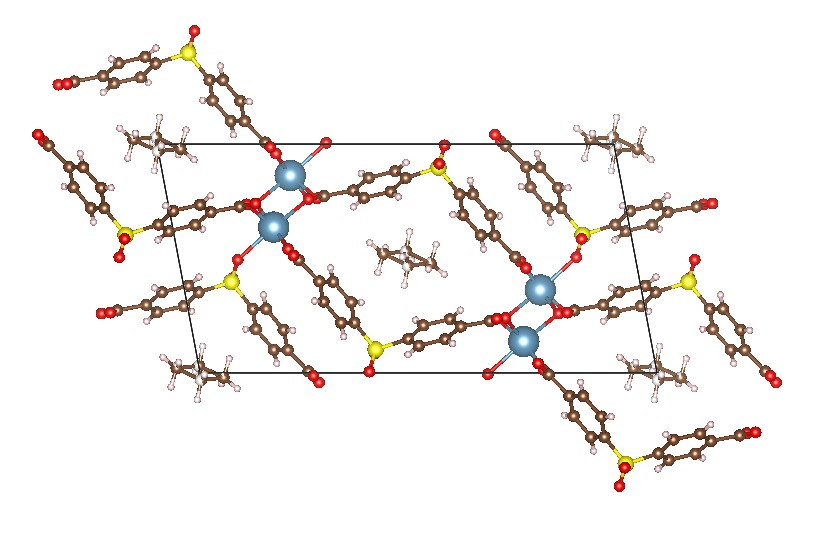
\includegraphics[height=0.6\textwidth]{figures/6-perspectives/QUXRUY.jpg}
    \caption{\texttt{QUXRUY}}\label{fgr:QUXRUY}
  \end{subfigure}
  \caption{ An illustration of the effect of the orientation of hexane inside a SBMOF-1-like material. In \texttt{QUXRIM} (a), the carbon atoms are oriented towards the S atoms, whereas in \texttt{QUXRUY} (b) they are oriented towards the Ca atoms. This difference in the orientation could explain the different structural properties of the materials reported in Table~\ref{table:sbmof}. Color code: brown for C, white for H, red for O, cyan for Ca, yellow for S. The structure visualizations are generated using the VESTA software.\autocite{VESTA}}\label{fgr:ads_config}
\end{figure}

Now that the adsorbate effects have been fully characterized on a few example configurations, it is easier to understand the thought process that led to the identification of \texttt{KAXQIL} as a candidate for Xe/Kr separation. The \texttt{KAXQIL} structure actually represents the material loaded by water with large pores, which enables a good interaction with a large molecule like xenon. For this reason, it was identified as a top selective material. However, when it was experimentally tested for low-pressure adsorption using the Henry constant, it is most likely that the pores are not stretched, which implies lower Henry constants than expected. The structures \texttt{UQEFAZ} or \texttt{KAXQOR} seem to provide a better description of this low-pressure case since the experimental selectivity values are much more consistent with their theoretical selectivity values. 

To confirm this hypothesis, a high-loading Xe/Kr binary mixture adsorption uptake would need to be measured. If xenon is highly represented in the adsorbent material, then the structure would be much more favorable to xenon adsorption, hence increasing the selectivity value closer to the theoretically predicted one. This also highlights a composition effect; if the initial mixture has a low xenon content, the structure would most likely have narrower pores, which could decrease the selectivity. By changing the composition of the binary mixture, this effect could also be measured experimentally if the initial hypothesis on the adsorbate-induced flexibility is correct.

This method could be generalized to other systems by screening for materials with a similar chemical composition and topology, for example. However, finding structures in very different adsorption conditions is not always possible due to biases in research focus. To overcome these limitations, these structures could be either experimentally generated when a material seems interesting to see if flexibility plays a role in the adsorption process, or computationally generated by running structure optimizations on loaded structures. Either way, this new approach to flexibility seems complementary to the ones mentioned previously as it seems to have a similar (or slightly higher due to the adsorbate) computational cost as the Witman approach, while avoiding the computationally prohibitive calculation (in a screening) presented by Bousquet et al.\autocite{Bousquet2012} 


\subsubsection{Diffusion in a flexible environment}

\begin{figure}[ht]
  \centering
  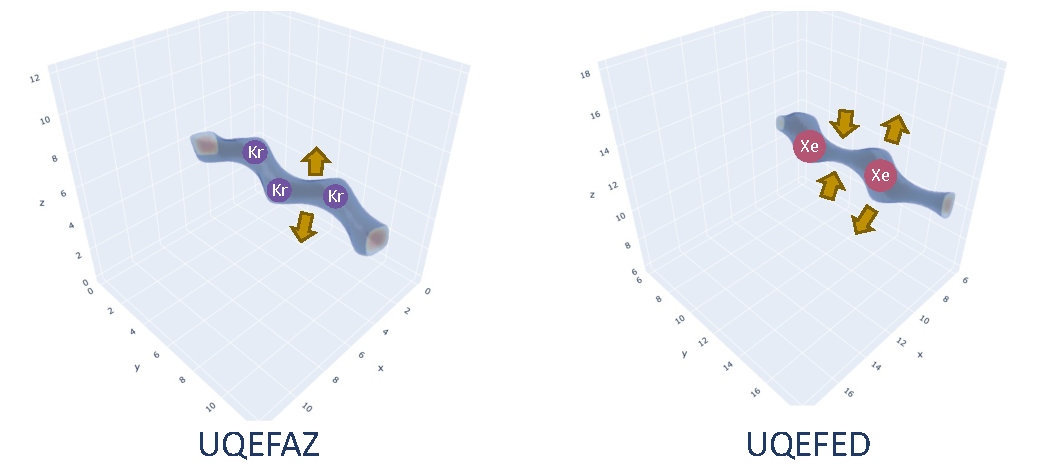
\includegraphics[width=0.8\textwidth]{figures/6-perspectives/KAXQIL_stretch.pdf}
  \caption{ Visualization of the pore size stretching effect using the GrAED algorithm. The xenon increases the LCD value while diminishing the PLD value. }\label{fgr:stretch}
\end{figure}

Guest transport can also be modulated by the adsorbate-induced flexibility of SBMOF-1. Depending on the structural configuration of the material, the diffusion coefficient becomes limiting only for some configurations of the material: it is equal to $3\times10^{-8}$~\si{\square\cm\per\s} for \texttt{KAXQIL} and $1\times10^{-11}$~\si{\square\cm\per\s} for \texttt{UQEFED} (Table~\ref{table:sbmof}). This lower diffusion coefficient can be explained by the change in PLD value, the channel bottleneck diameter, induced by the stretching illustrated in Figure~\ref{fgr:stretch}. For a material predominantly loaded with krypton molecules, the diffusion channel is significantly broader, which explains the much higher diffusion coefficient of xenon ($5\times10^{-6}$~\si{\square\cm\per\s}). Although the xenon adsorbate does not diffuse freely in the structure, the diffusion is much less obstructed than in the previous material configuration of SBMOF-1 (\texttt{UQEFED}). The Figure~\ref{fgr:stretch} suggests that the SBMOF-1 material changes its pore configuration according to the shape and size of the atoms loaded inside, and these induced deformations lead to significantly different separation performances.

Now having identified two completely distinct diffusion behaviors, these results can be extrapolated to hypothetical conditions. For instance, if there is a relation between the quantity of xenon inside the pores and the structural similarity towards \texttt{UQEFED}, then the material could kinetically limit the adsorption of xenon at high loading of xenon. In other words, adsorbing xenon at higher xenon loading values may be kinetically more challenging. However, at lower xenon loading, there are no diffusion limitations, as indicated by the steep mass transfer zone observed in the breakthrough curve of xenon in Figure~\ref{fgr:sbmof_breakthrough}. By connecting these results to the influence of flexibility on transport properties and the adsorption process, it can be inferred that xenon adsorption is thermodynamically much more favorable at higher xenon loading. There is a thermodynamics/kinetics trade-off, as articulated in the previous chapter on \texttt{KAXQIL}. Since \texttt{KAXQIL} and \texttt{UQEFED} are structurally similar, the combination of diffusion limitation and high selectivity can be extended to the xenon-loaded structure (\texttt{UQEFED}), as confirmed by the diffusion coefficient and selectivity values reported in Table~\ref{table:sbmof}. From an industrial perspective, the inclusion of transport effects in the analysis reveals additional costs associated with adsorbing xenon at high loading values, if this theoretical study is validated by experiments.

By employing simple simulation methods (Widom insertion and MD) on rigid structures, the effects of flexibility on both the adsorption and transport properties were probed using experimentally resolved structures under different adsorption conditions. These results shed light on the experiment-theory discrepancies and provides insights into similar problematic systems. In this study, the experimental data published on the SBMOF-1 structure was used, but such resources may not always be available for other systems. In such cases, generating data using experiments or simulations could be necessary. If generalized, this approach would enable its automatic application to a series of structures, paving the way for ``flexibility-aware'' screenings in the future. Recognizing the importance of both flexibility and transport effects, other studies have attempted to incorporate both in a small-scale screening process.\autocite{Stanton_2022} These authors used a flexible forcefield and MD simulations to determine the diffusion coefficient, while adsorption performance was assessed through DFT calculations at the adsorption site. The main issue of this method is its computational cost, but it can serve as an alternative solution to the one introduced here, when no prior knowledge is available on the structure’s flexibility. 

\section{Noble gas polarizability}

The last effect that could greatly influence adsorption performance is the level of theory behind the modeling of interaction energy. In most screening studies, (our group included), very low-level classical theories are commonly utilized to describe guest--host interactions due to their low computational cost. To improve the accuracy of descriptions, some studies focus on a few specific structures and use higher levels of theory such as DFT calculations. However, the computational cost associated with these methods is prohibitive for high-throughput screenings.

Prior to exploring higher-cost methods, it is essential to first identify the limitations of molecular modeling in current screening methodologies. This work is motivated by recent advancements in experimental design of nanoporous materials for Xe/Kr separation. The most selective materials are based on highly polar groups or exposed open-metal sites.\autocite{Li_2019,Pei_2022} The polarization phenomenon is, therefore, central to these materials, but it cannot be adequately described by a simple Lennard-Jones potential, particularly when induced by high partial charge values.

For this reason, it is necessary to develop a polarizable forcefield that incorporates the effect of the surrounding partial charges into the guest--host interactions. The difference in polarizability between xenon and krypton may lead to the emergence of new materials. The ranking of the best materials obtained through this type of screening would differ significantly from the standard ranking. This section will present the problem of current methodologies through an experiment-theory comparison and explore alternative methodologies that can account for polarization in the commonly employed Lennard-Jones potentials.

\subsection{Problem definition}

\begin{figure}[ht]
  \centering
  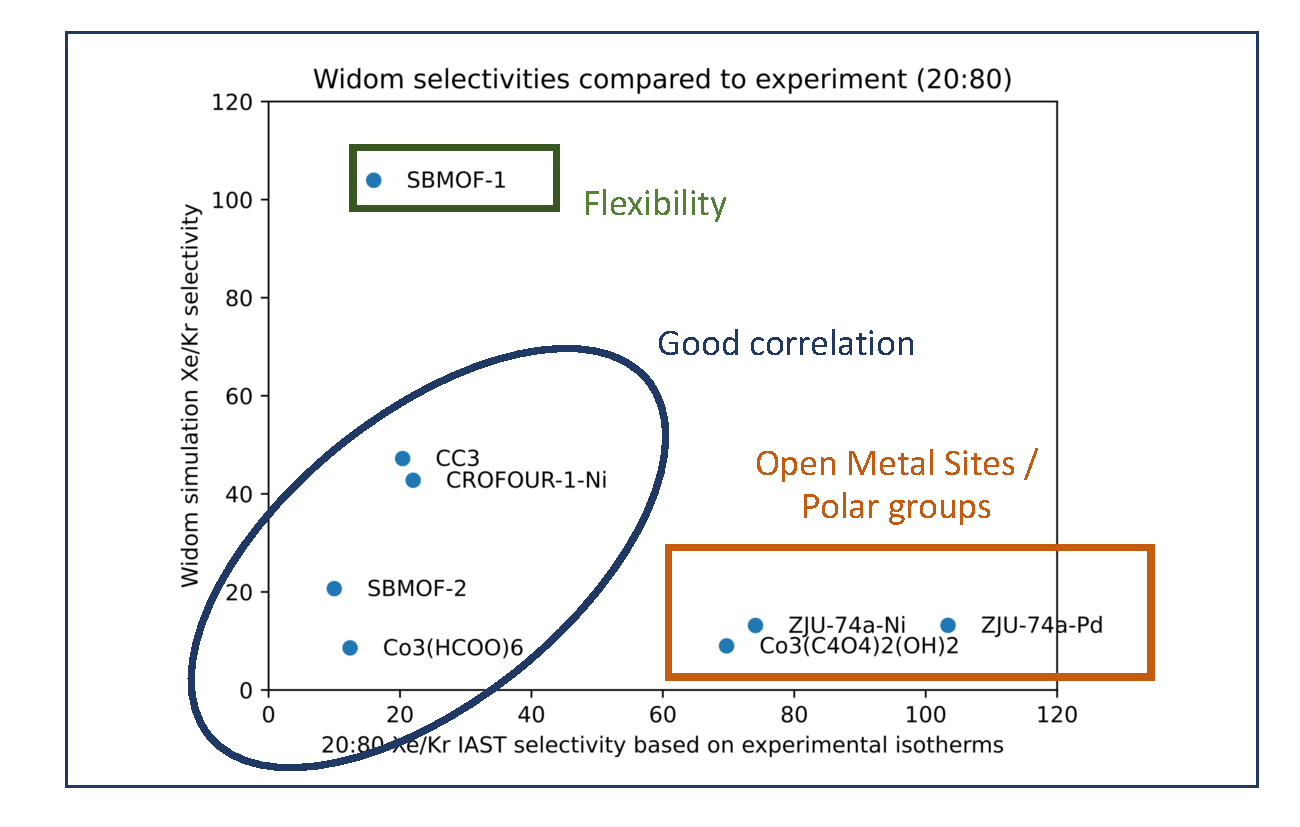
\includegraphics[width=0.7\textwidth]{figures/6-perspectives/exp_theory_discrepancies.pdf}
  \caption{ Comparison between the selectivity values obtained experimentally and computationally. The structures are split into three categories depending on the difference between experiments and theory. The case of SBMOF-1 can be attributed to its flexibility. The discrepancies between the materials in the lower right correspond to the ones introduced by Li et al.\ and Pei et al.,\autocite{Li_2019,Pei_2022} and the difference can be explained by the polarization that is not included in the level of theory considered. }\label{fgr:exp_theory_discrepancy}
\end{figure}

If the selectivity of good materials for xenon/krypton separation that are often presented in the literature is considered, the materials named \ce{Co3(HCOO)6},\autocite{Wang_2014} CC3,\autocite{Chen_2014} SBMOF-2,\autocite{Chen_2015} CROFOUR-1-Ni,\autocite{Mohamed_2016}  SBMOF-1,\autocite{Banerjee_2016} \ce{Co3(C4O4)2(OH)2}\autocite{Li_2019} and ZJU-17a\autocite{Pei_2022} often appear as top separation materials. When the selectivity values obtained through a Widom insertion with the UFF forcefield are compared to the experimental values as shown in Figure~\ref{fgr:exp_theory_discrepancy}, a good correlation is generally observed. However, in some cases like SBMOF-1, the difference observed could be explained by other effects (see previous section on flexibility). In other cases, the difference could be explained by the polarization effect that was not taken into account. To better understand this phenomenon, this study will focus on two papers that found record-breaking Xe/Kr selectivity values based on polar hydroxyl groups and open metal sites.

The first paper of Li et al.\autocite{Li_2019} published in 2019 introduced a squarate-based MOF with a Xe/Kr selectivity of $69.7$ for a 20:80 binary mixture estimated by the ideal adsorbed solution theory (IAST)\autocite{Cessford_2012}. The authors explained this outstanding xenon affinity by two factors: a pore size close to the kinetic diameter of a xenon and the stabilization effect of the hydroxyl group. DFT calculations determined binding energies of the order of \SI{44.1}{\kJ\per\mole} for xenon and \SI{33.7}{\kJ\per\mole}, which suggests a separation process of enthalpic nature (usually the case for highly selective materials). Due to the high electronegativity of the oxygen atom, the hydroxyl group pointing to the pore center (as illustrated in Figure~\ref{fgr:jacs_li_str}) interacts strongly with the xenon through a permanent dipole--induced dipole interaction (introduced in the section~\ref{sct:interaction}). This high xenon affinity is illustrated by the experimental isotherms in Figure~\ref{fgr:jacs_li_isotherm}. On the other hand, the pore wall creates unidimensional channels that present adsorption pores with a \SI{4.1}{\angstrom}$\times$\SI{4.3}{\angstrom} size, which is very close to the xenon kinetic diameter of about \SI{4.0}{\angstrom}. 

\begin{figure}[ht]
  \centering
  \begin{subfigure}[b]{0.34\textwidth}
    \centering
    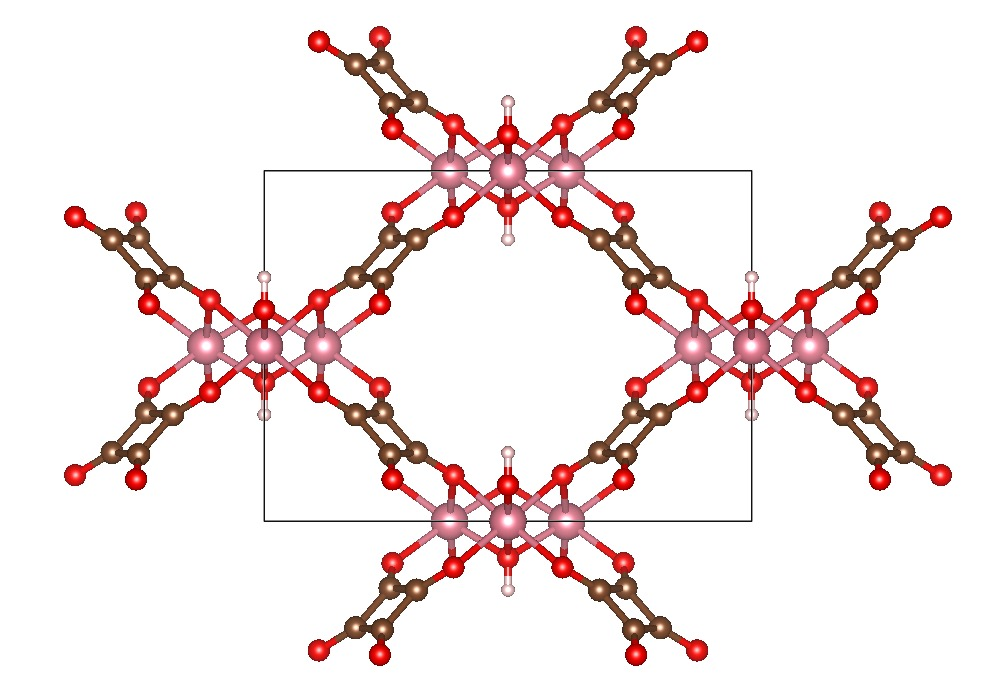
\includegraphics[width=\textwidth]{figures/6-perspectives/jacs_li.jpg}
    \caption{VESTA visualization\autocite{VESTA}}\label{fgr:jacs_li_str}
  \end{subfigure}
  \hfill
  \begin{subfigure}[b]{0.34\textwidth}
    \centering
    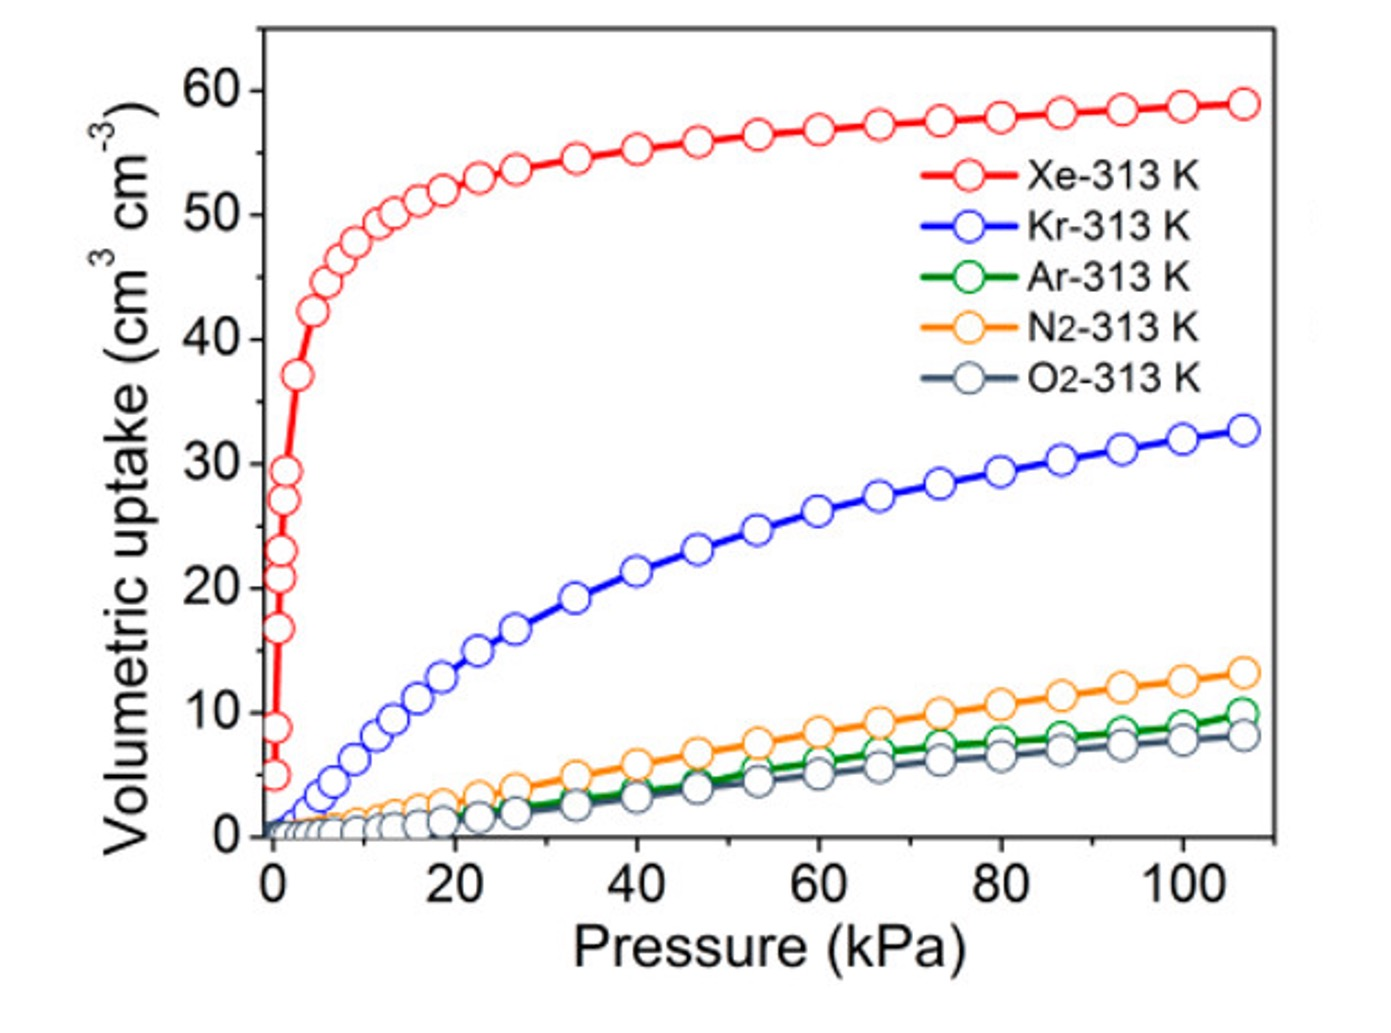
\includegraphics[width=\textwidth]{figures/6-perspectives/jacs_li_isotherm.jpg}
    \caption{Adsorption isotherms}\label{fgr:jacs_li_isotherm}
  \end{subfigure}
  \hfill
  \begin{subfigure}[b]{0.25\textwidth}
    \centering
    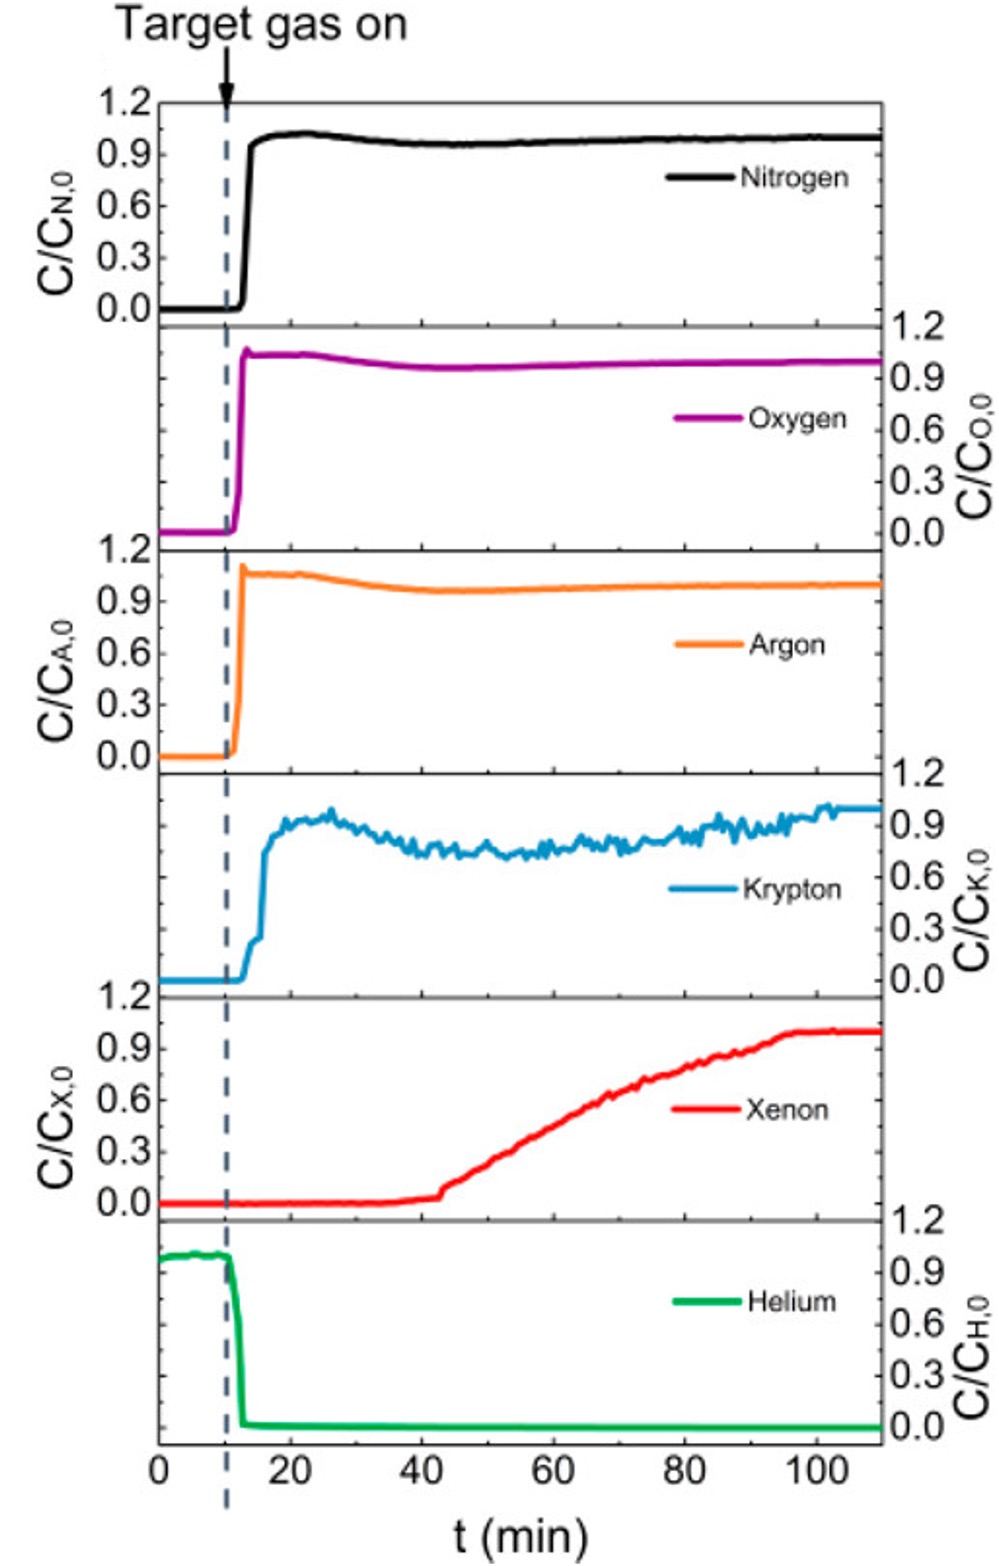
\includegraphics[width=\textwidth]{figures/6-perspectives/jacs_li_breakthrough.jpg}
    \caption{Breakthrough curves}\label{fgr:jacs_li_breakthrough}
  \end{subfigure}
  \caption{ (a) Representation of the squarate-MOF \ce{Ce3(C4O4)2(OH)2} structure with the color code: brown for C, white for H, red for O, pink for Co. The hydroxyl group, to which the high Xe/Kr selectivity is attributed, is visible in the structure. (b) Mono-component adsorption isotherm measured experimentally for Xe, Kr, Ar, \ce{N2} and \ce{O2}. (c) Experimental breakthrough curves for a gas mixture with 400 ppm Xe and 40 ppm Kr balanced with dry air. Reprinted with permission from Ref.~\cite{Li_2019} copyright \copyright\ 2019 American Chemical Society. }\label{fgr:jacs_li}
\end{figure}

Finally, the breakthrough experiment data (Figure~\ref{fgr:jacs_li_breakthrough}) reveals a relatively slow release of xenon in the mass transfer zone, which suggests a relatively low xenon diffusion coefficient in this material. The diffusion limitation seems to occur even at very low xenon partial pressure (400 ppm) in this material. This was not the case for SBMOF-1, as the xenon breakthrough curve was much steeper (rapid mass transfer) as shown in Figure~\ref{fgr:sbmof_breakthrough}. To have a closer look at the transport effect in this squarate-MOF, similar simulations should be performed as for SBMOF-1 with a polarizable forcefield.

In the second work,\autocite{Pei_2022} Pei et al.\ introduced two Hofmann-type MOFs with record-breaking Xe/Kr selectivity values. The first Co/Ni-based MOF, called ZJU-74a-Ni, has an estimated IAST selectivity of $74.1$ for a Xe/Kr binary mixture of composition 20:80 at \SI{1}{\bar} and \SI{298}{\kelvin}, while the second Co/Pd-biased MOF, ZJU-74a-Pd, displays a selectivity of $103.4$ in the same ambient-pressure conditions. As shown in Figure~\ref{fgr:jacs_pei_iast}, the IAST selectivity of ZJU-74a-Pd is not always that high and can decrease to $30$ at very low-pressure conditions. The authors attribute the record-breaking selectivity values of these materials by a size close to the kinetic diameter of xenon and, above all, the increased interaction with the open metal site, either the nickel or the palladium atoms. The Horvath–Kawazoe method provided a pore size of \SI{4.0}{\angstrom} and \SI{3.8}{\angstrom} for the Ni and Pd-based MOFs, respectively. The xenon binding energy was evaluated to be around \SI{38}{\kJ\per\mole} for ZJU-74a-Ni using a UFF-based method. It should be noted that this value is much lower than the one obtained for the squarate-based MOF. Further investigations with a DFT method are required to determine the real binding energy for this material due to its higher experimental performance compared to the computational result. 

\begin{figure}[ht]
  \centering
  \begin{subfigure}[b]{0.34\textwidth}
    \centering
    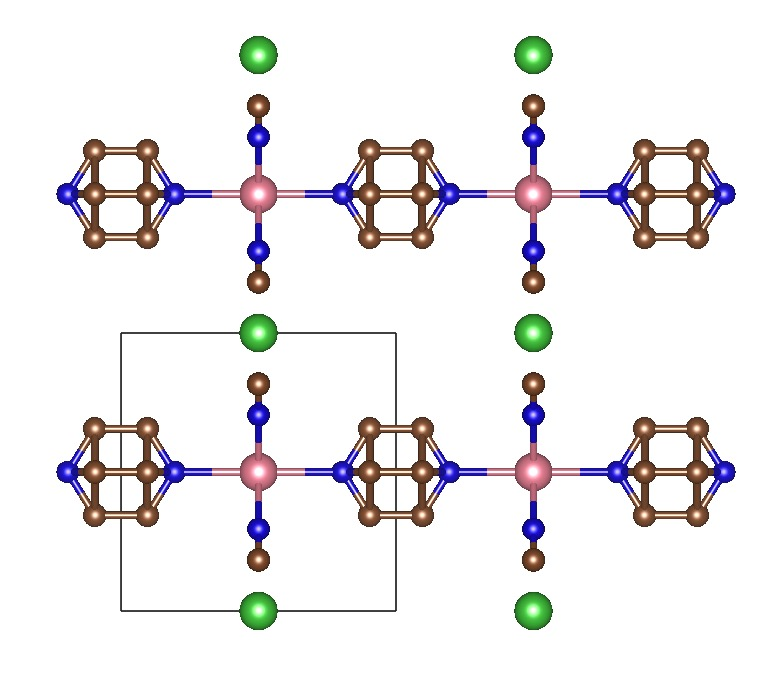
\includegraphics[width=\textwidth]{figures/6-perspectives/jacs_pei.jpg}
    \caption{VESTA visualization\autocite{VESTA}}\label{fgr:jacs_pei_struc}
  \end{subfigure}
  \hfill
  \begin{subfigure}[b]{0.34\textwidth}
    \centering
    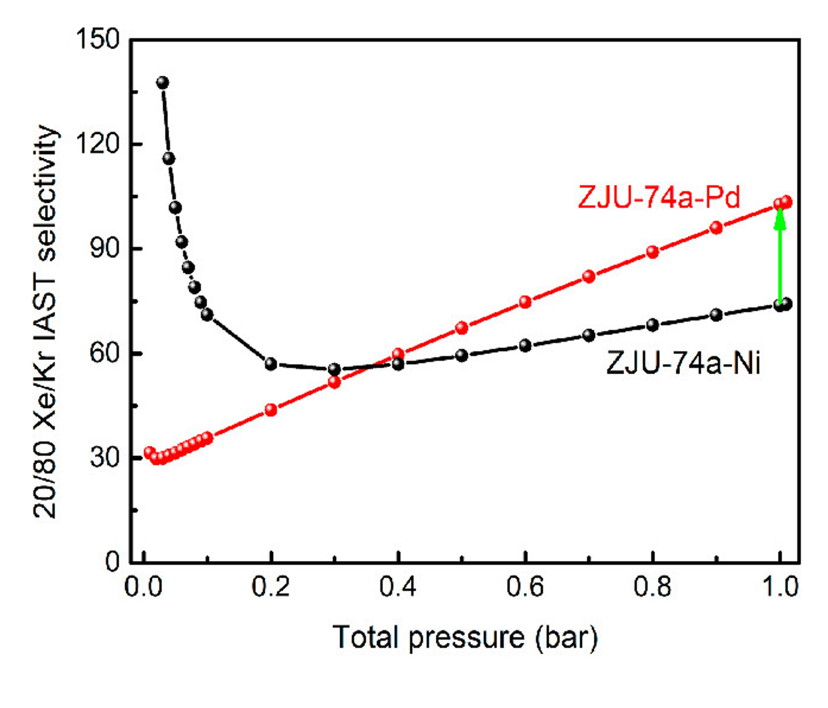
\includegraphics[width=\textwidth]{figures/6-perspectives/jacs_pei_iast.jpg}
    \caption{IAST selectivity}\label{fgr:jacs_pei_iast}
  \end{subfigure}
  \hfill
  \begin{subfigure}[b]{0.25\textwidth}
    \centering
    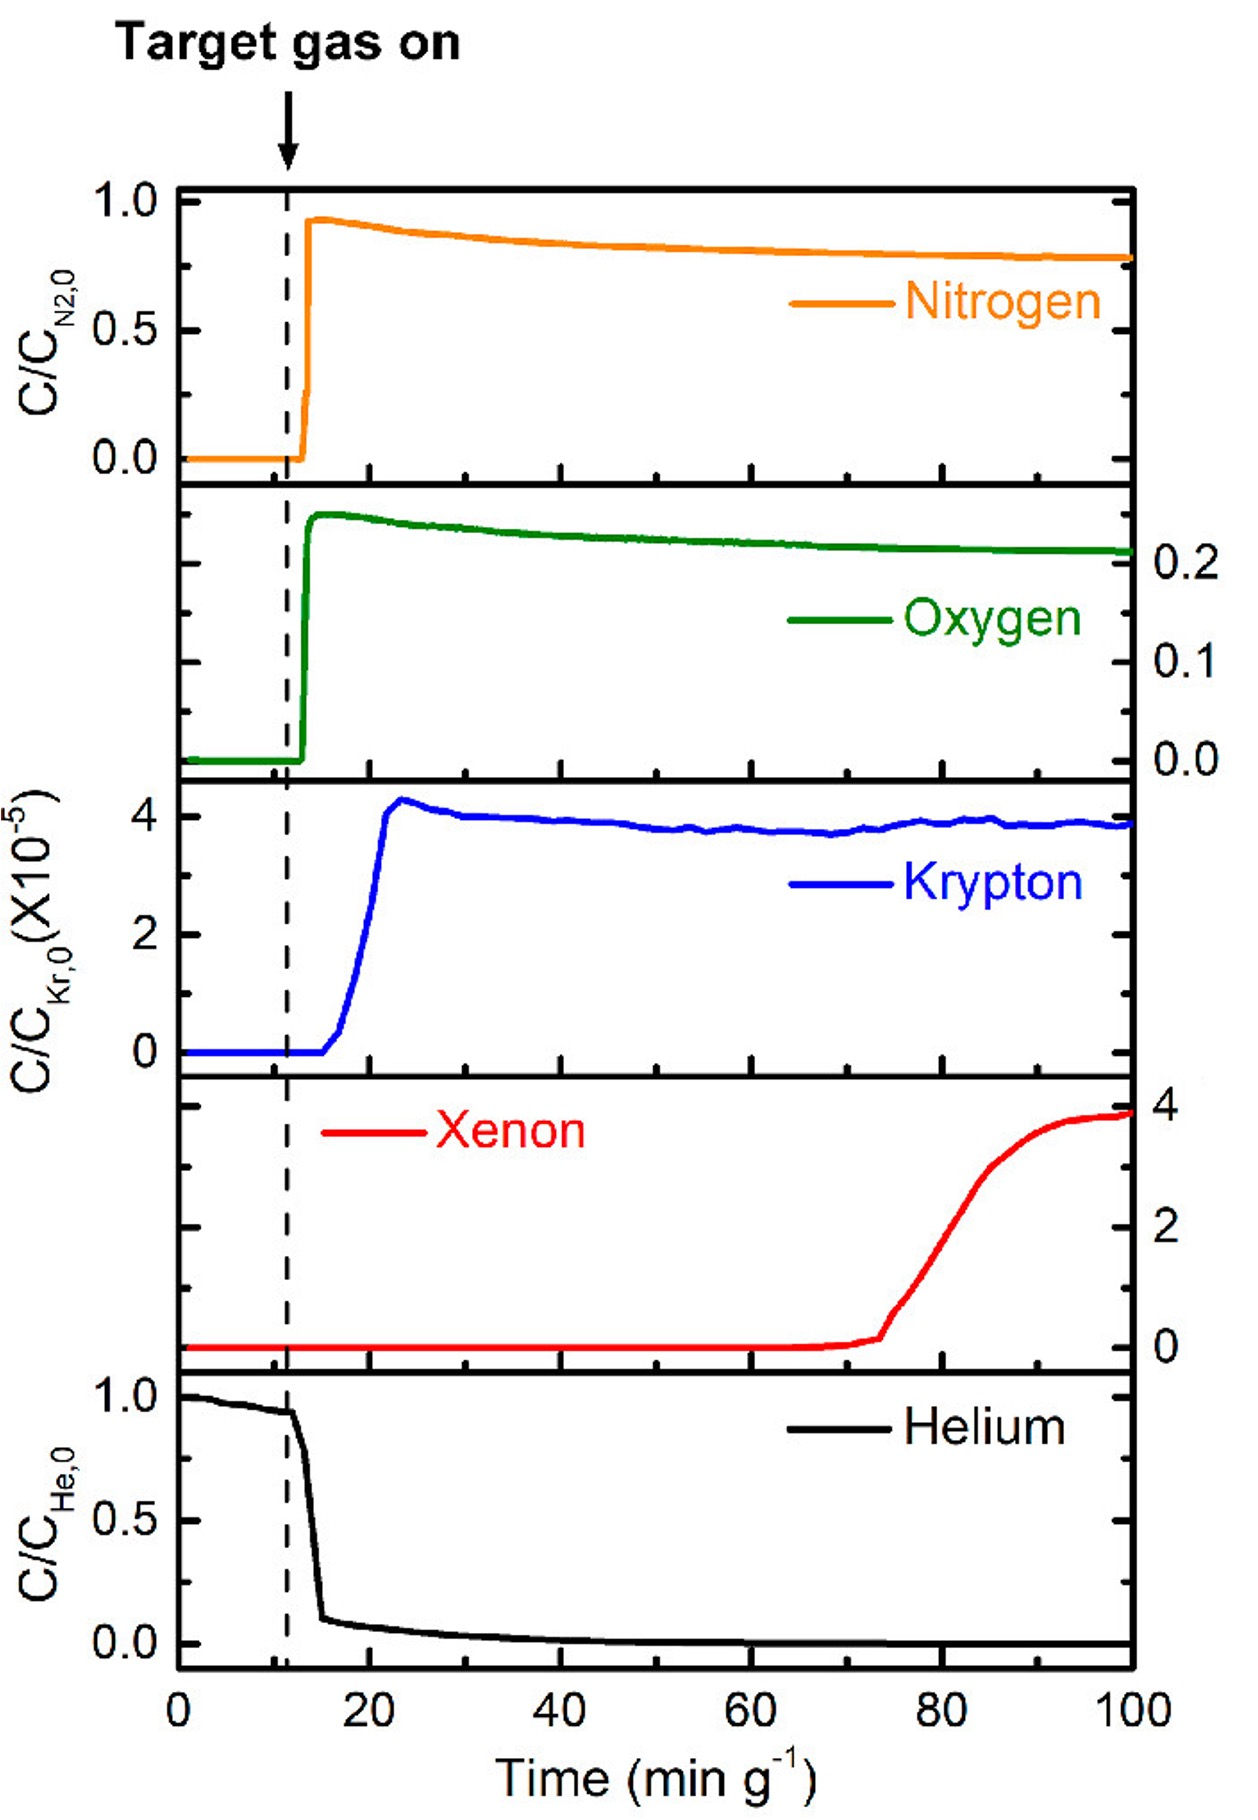
\includegraphics[width=\textwidth]{figures/6-perspectives/jacs_pei_breakthrough.jpg}
    \caption{Breakthrough curves}\label{fgr:jacs_pei_breakthrough}
  \end{subfigure}
  \caption{ (a) Representation of the ZJU-74a-Ni structure with the color code: brown for C, white for H, red for O, pink for Co, green for Ni. We can see the open metal sites or coordinatively unsaturated nickel metals that could interact with an adsorbate in the center of the pore. (b) Selectivity values at different pressure conditions for a 20:80 Xe/Kr binary mixture calculated by the IAST theory. (c) Experimental breakthrough curves of a gas mixture with 400 ppm Xe and 40 ppm Kr balanced with dry air in ZJU-74a-Pd. Reprinted with permission from Ref.~\cite{Pei_2022} copyright \copyright\ 2022 American Chemical Society.}\label{fgr:jacs_pei}
\end{figure}

Finally, the breakthrough experiment suggests a relatively slow mass transfer in the material. However, when compared to the squarate-based material under similar conditions, the mass transfer seems to be much faster, as the mass transfer zone is shorter. Therefore, it can be inferred that ZJU-74a-Pd is probably a better material than \ce{Co3(C4O4)2(OH)2} due to its superior adsorption and transport properties for Xe/Kr separation. In comparison to SBMOF-1 with a relatively low xenon partial pressure, a slight diffusion limitation phenomenon seems to be present. The retention of xenon is, on the other hand, longer in ZJU-74a-Pd (around \SI{70}{\s}) than in SBMOF-1 (around \SI{65}{\s}). More information regarding the ambient-pressure selectivity of SBMOF-1 is necessary to complete the comparison.
This material is also noteworthy for its robustness in different pH, humidity and radiation conditions, making it an ideal choice for capturing xenon produced by nuclear reactions in nuclear installations.

These two studies clearly demonstrate the failure of current screening methodologies in identifying materials whose performance relies on polarization effects. The next and final discussion will introduce some methods for incorporating polarization into Lennard-Jones potentials that could be used in a screening procedure.

\subsection{Studying the polarization}

The physical reason behind the consideration of the polarization effect for xenon/krypton separation is to exploit the difference in polarizability between Xe (\SI{4.0}{\cubic\angstrom}) and Kr (\SI{2.5}{\cubic\angstrom})\autocite{Olney1997} to its full potential. Seen from a broad perspective, the order of magnitude of the induction energy is actually higher than other standard van der Waals energies, as explained in Section~\ref{sct:interaction}. For instance, the ion-induced dipole interaction is reported to range between 40--600~\si{\kJ\per\mol}. In the case of ZJU-74a-Ni, the Ni\ex{2+}---Xe---Ni\ex{2+} interaction originates from selectivity, which corresponds to this specific type of interaction and predominantly explains the experimental selectivity values. Incorporating polarization into the screening procedure has the potential to completely alter the obtained structures and the types of interactions at play.

Bearing this in mind, Becker et al.\ carried out an interesting study on a series of MOF materials with a high density of open-metal sites, the M-MOF-74 with M = Co, Cr, Cu, Fe, Mg, Mn, Ni, Ti, V, and Zn.\autocite{Becker_2017} By introducing a potential induced by the surrounding partial charges to a modified LJ potential, the authors successfully replicated the experimental isotherm data for \ce{CO2} and \ce{CH4} adsorption on this series of MOFs. They also showed the inadequacy of the standard UFF force field in describing the adsorption behavior of \ce{CO2} on the open-metal sites, thereby overlooking a highly adsorptive site at infinite dilution.

This novel method is based on the procedure developed by Lachet et al.\autocite{Lachet_1998}, which considers the induced dipole method, where the induction energy $U\e{ind}$ is expressed as follows:

\begin{equation}
  U\e{ind} = -\frac{1}{2} \sum_{i=1}^{N} \boldsymbol{\mu}_i \cdot \mathbf{E}_i^0
\end{equation}
where $\boldsymbol{\mu}_i$ is the induced dipole, and $\mathbf{E}_i^0$ is the electric field created by the surrounding atoms' partial charges on the particle $i$. Since the induced dipole also interacts with the surrounding induced dipoles $j$$\neq$$i$, the induced dipole is usually calculated using a back-propagation algorithm as described in the Ref.~\cite{Lachet_1998}. However, it was found that back-propagation accounts for less than {5\%} of the total induction energy. For this reason, the equation can be simplified by considering only the interaction between the induced dipole and the surrounding electric field, without taking into account induced-dipole--induced-dipole interactions. Moreover, skipping the back-propagation step saves valuable computation time during screening. The induction energy can then be expressed as follows:

\begin{equation}
  U\e{ind} = -\frac{1}{2} \sum_{i=1}^{N} \alpha_i {\left\lvert\mathbf{E}_i^0\right\rvert}^2
\end{equation}

Since a portion of the induction energy is already incorporated into the Lennard-Jones potential, the authors rescaled the LJ parameters to eliminate the induction part from the LJ energy. This part appears to be system-dependent and may be debatable since it allows for fitting to experimental data without solid theoretical justification. To address this properly, a force field should be designed around this concept to fine-tune the LJ parameters based on specific experimental data, similar to standard force field development practices.

By customizing this method for xenon/krypton separation, it may be possible to conduct screenings that yield materials comparable to ZJU-74a-Pd. Further optimization of the process can be achieved by narrowing down the materials' selection through restrictions on pore size and the presence of open metal sites within a database. Subsequently, the restricted material list can be evaluated using higher-level methods like the ones described in this chapter.


\OnlyInSubfile{\printglobalbibliography}

\end{document}
